\documentclass[text04.tex]{subfiles}
\begin{document}
%2083
\newpage
\section{プログラミングの応用}

\subsection{サンプルフォルダを準備しよう}

上にあるバーのアイコンからファイルマネージャーを開いてみましょう。

\begin{figure}[H]
    \begin{center}
      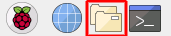
\includegraphics[keepaspectratio,width=5.898cm,height=1.242cm]{../../asset/image/s_filemanager.png}
      \caption{ファイルマネージャーを開くアイコン}
    \end{center} .
\end{figure}

これからHSPで使うことのできるサンプルプログラムをコピーしてもらいます。「/home/ユーザー名」のフォルダに、「sample」フォルダをコピーすることから始めます。

まず、「/usr/local/share/OpenHSP」という場所を開いてみましょう。

この中に、「sample」という名前のフォルダがあります。これから、この「sample」というフォルダを自分の作業フォルダにコピーします。

「sample」という名前のフォルダ上でマウスの右クリックを押して「コピー」を選んでください。


\begin{figure}[H]
    \begin{center}
      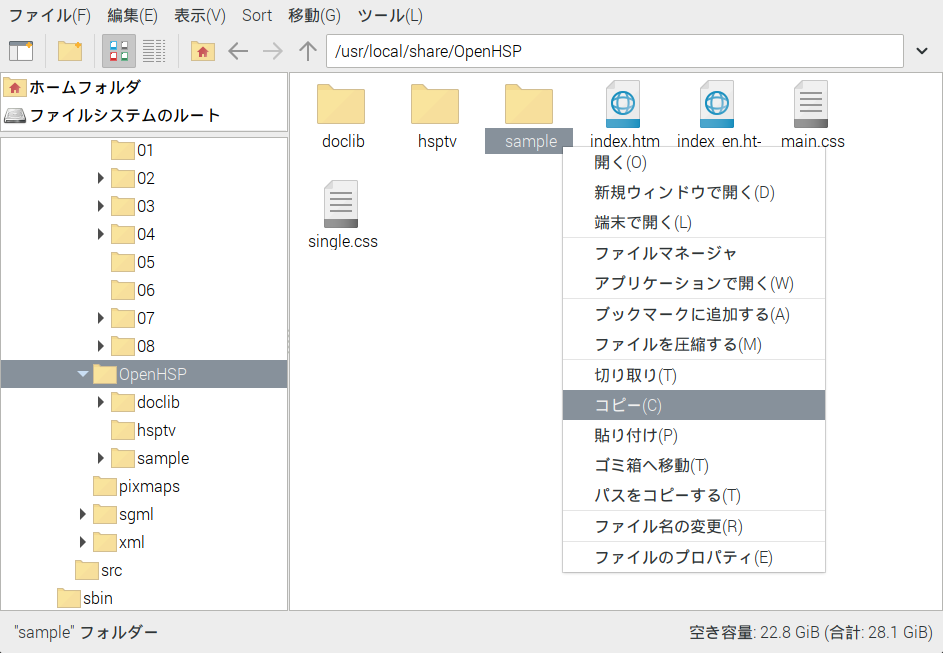
\includegraphics[keepaspectratio,width=11.232cm,height=8.424cm]{../../asset/image/s_ome04e.png}
      \caption{sampleフォルダでコピーを選ぶところ}
    \end{center}
\end{figure}

この後、コピーしたい場所を選びます。コピー先の場所は、「/home/ユーザー名」のフォルダになります。

コピー先の場所を開いたら、何もない場所でマウスの右クリックを押して「貼り付け」を選んでください。

これで先ほどの「/usr/local/share/OpenHSP/sample」フォルダが、「/home/ユーザー名/sample」にコピーされます。

ファイルには、さまざまなプログラムとデータが入っています。

すべてのファイルを\ruby{紹介}{しょう|かい}できませんが、\ruby{興味}{きょう|み}がある人は時間がある時に読み込んで動かしてみましょう。

%2146


%2146
\newpage
\subsection{\ruby{立体的}{りっ|たい|てき}な絵を出すには}

いままで\ruby{平面的}{へい|めん|てき}な絵を使ってきました。いわゆる「2D」と呼ばれる\ruby{表現}{ひょう|げん}です。

ゲームやCGでは、立体的な「3D」表現が使われています。実際に、立体的な絵を出すプログラムを動かしてみましょう。


先ほどコピーした「/home/ユーザー名/sample」フォルダの中からプログラムを読み込みます。

ファイル→「開く」メニューから「/home/ユーザー名/sample/hgimg4」内の「light\_test3.hsp」を読み込んでください。


\begin{lstlisting}[caption=light\_test3.hspのプログラムの一部]
#include "hgimg4.as"

title "HGIMG4 Test"

    ;       ポイントライト色変化テスト
    ;       マウス/タッチドラッグでカメラを動かすことができます
    ;
    randomize

    gpreset
    gpresetlight 1,1                        ; ポイントライトを1個追加する

    setcls CLSMODE_SOLID, $404040           ; 背景色

    setcolor GPOBJ_LIGHT, 0.5,0.5,0.5       ; 標準ライトカラーを設定
    setdir GPOBJ_LIGHT, 0.2,0.2,0.2         ; 標準アンビエントカラーを設定

    ;       箱をライトとして設定します
    ;       何もないモデルをライトにする場合はgpnullで生成してください
    gpbox id_model, 0.5, $ffffff            ; 箱ノードを生成する
    gplight id_model, GPOBJ_LGTOPT_POINT,10 ; ポイントライトとして設定する
    setcolor id_model, 1,1,1                        ; ライトカラーを設定
    gpuselight id_model                             ; ポイントライトを使用する

    ;       モデルをたくさん配置する
    i=-1
    mdx=10:mdz=10                           ; X,Z方向の個数
    px=20.0/mdx:pz=20.0/mdz                 ; 間隔を計算する
    z=-10.0                                 ; 配置開始Z座標
    repeat mdz
    x=-10.0                                 ; 配置開始X座標
    repeat mdx
        if i<0 {
            ;gpload id_base,"res/duck"; モデル読み込み

\end{lstlisting}

[F5]キーで実行すると絵が動きます。

3D表現の画面を出す場合でも、プログラミングの方法は変わりません。ただし、今まで「横」「縦」という2つの\ruby{軸}{じく}があったものが、「横」「縦」「\ruby{奥行}{おく|ゆ}き」という3つの軸に増えて、絵を出す方法も\ruby{複雑}{ふく|ざつ}になります。

\begin{figure}[H]
    \begin{center}
      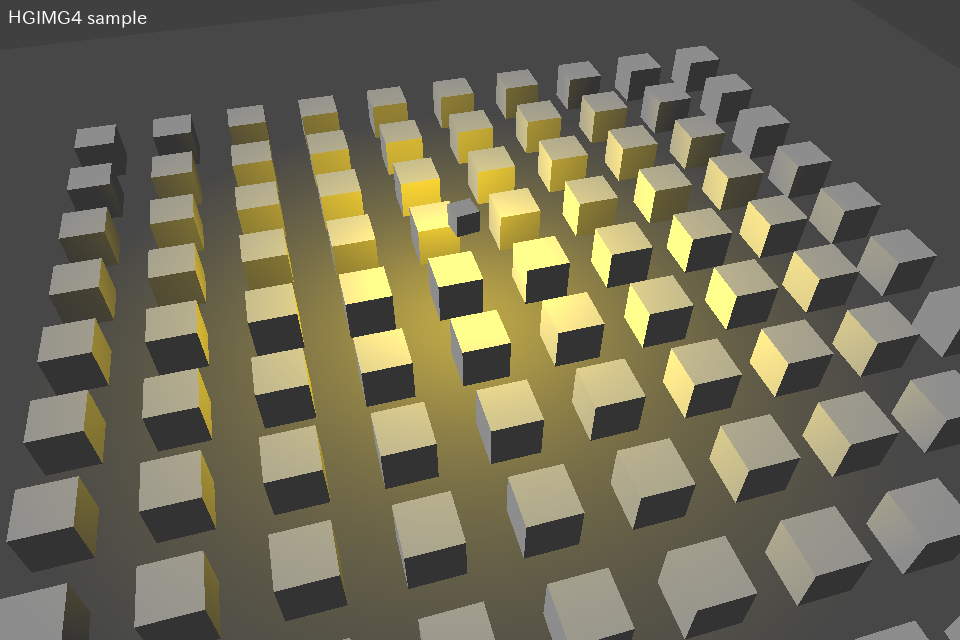
\includegraphics[keepaspectratio,width=10.971cm,height=8.229cm]{../../asset/image/s_lighttest3.png}
      \caption{light\_test3.hspの実行画面}
    \end{center} .
\end{figure}


変数や条件判断といった基本的な\ruby{要素}{よう|そ}は変わらないので、まず「2D」のやり方をよく覚えて、さらにそこからステップアップすることをおすすめします。

もう1つ、立体的なキャラクターを出すプログラムを見てみましょう。


ファイル→「開く」メニューから「/home/ユーザー名/sample/pronama3d」内の「pronama2.hsp」を読み込んでください。

[F5]キーで実行するとプロ生ちゃんというキャラクターがダンスする画面になります。


\begin{figure}[H]
    \begin{center}
      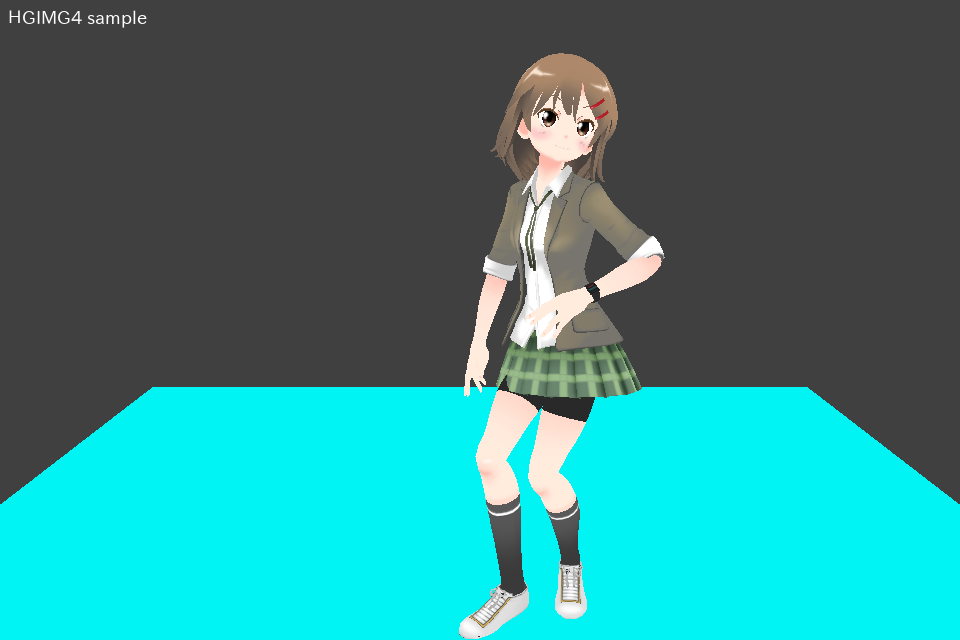
\includegraphics[keepaspectratio,width=10.971cm,height=8.229cm]{../../asset/image/s_pronama2.png}
      \caption{pronama2.hspの実行画面}
    \end{center}
\end{figure}

立体的な絵は、GIMPのような絵を描くツールではなく、3Dグラフィックツールと呼ばれる、形そのものを細かく決めるツールによって作られています。これは、2Dの絵を描くよりもずっと難しい作業です。しかし、仕組みがわかって\ruby{学習}{がく|しゅう}すれば作れるものでもあるのです。


皆さんが使っているラズベリーパイは、スマホやPCと同じような3D表示にも\ruby{対応}{たい|おう}した\ruby{高性能}{こう|せい|のう}なコンピュータです。

応用によって\ruby{本格的}{ほん|かく|てき}なゲームも遊べますし、それを作りだすこともできることを覚えておいてください。


\begin{figure}[H]
    \begin{center}
      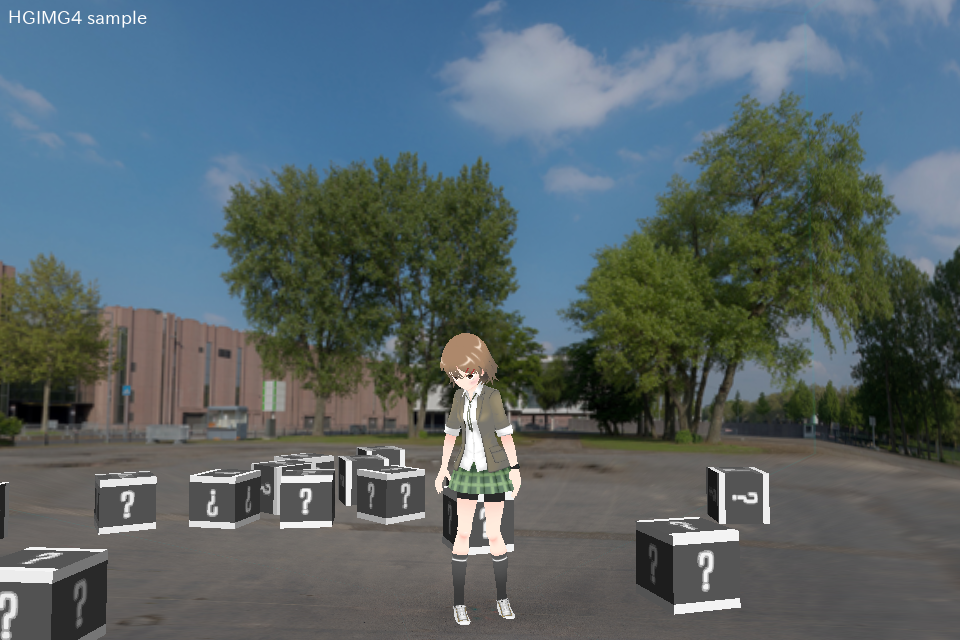
\includegraphics[keepaspectratio,width=10.834cm,height=7.514cm]{../../asset/image/s_pronamabox.png}
      \caption{背景とキャラクターを同時に出した画面}
    \end{center} .
\end{figure}

%2250
%2250
\newpage
\subsection{たくさんの絵を\ruby{同時}{どう|じ}に動かす}

\ruby{以前}{い|ぜん}に、変数に横・縦の位置を代入してpos命令で指定することで絵を動かすプログラムを実行しました。変数を使うことで、絵を動かしたり、条件判断ができることはわかりました。

でも、ゲームの中では、同時にたくさんの絵を動かしています。

たくさんの敵が出てきたり、ミサイルが同時に\ruby{発射}{はっ|しゃ}されたりします。これを変数で1つ1つ記憶させるためには、それだけ多くの変数を作る必要があります。

変数x、変数yが横・縦の位置を入れておくものだとして、もう1つまた変数x2、変数y2…など違う名前をつけなければなりません。

もし100個の絵を出すとすると、x100とかすごい数を書く必要があるのでしょうか…?


実は、これを簡単にできるような仕組みが用意されています。それが「\ruby{配列変数}{はい|れつ|へん|すう}」と呼ばれるものです。

変数はx,yなどの名前を付けた箱に数字を入れてありました。この箱に番号を付けて\ruby{管理}{かん|り}できるようにしたものが配列変数です。

変数xの1番目、2番目、3番目…といった感じで、変数の名前は同じで、番号ごとに違う内容を記憶させておくことができます。配列変数を使う時には、「(カッコ)」の中に番号を書きます。


\deschspsyntax{変数(番号)}

たとえば、変数xの1番目は、x(1)のように書きます。x(1)とx(2)は別々な数字を覚えさせることができます。後は、いままでの変数と使い方は変わりません。ですから、



\begin{lstlisting}[numbers=none]
x(1) = 100
x(2) = 200
x(3) = 400
\end{lstlisting}


のようにいくつも変数xの配列変数に代入することができます。

カッコの中の番号は、0から始まって好きな数まで入れていくことができます。この番号を\ruby{配列要素}{はい|れつ|よう|そ}と呼んでいます。番号は実は、数字だけでなく変数を使うことができます。つまり、

\begin{lstlisting}[numbers=none]
a=3
x(a) = 500
\end{lstlisting}

と書いた場合は、x(3)に500という数字が代入されます。

同じ変数に複数の値が入るということで、ちょっと難しいですが、これを使うことで同時に絵を動かすことができるようになります。

ファイル→「開く」メニューから「array.hsp」を読み込んでください。

[F5]キーで実行すると、同時に小さな絵が動きます。

\begin{figure}[H]
    \begin{center}
      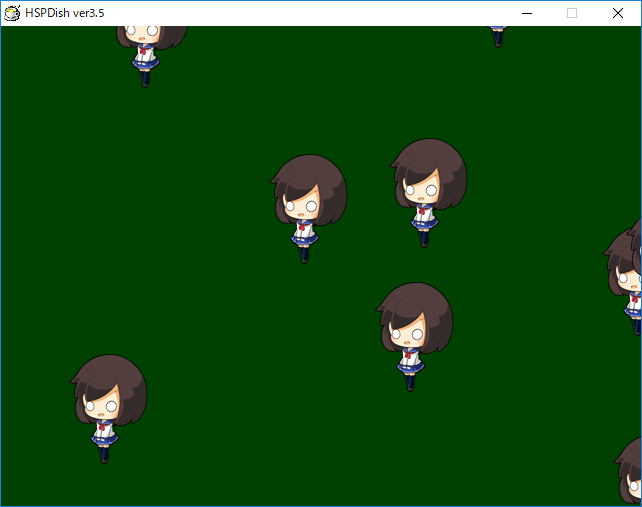
\includegraphics[keepaspectratio,width=8.811cm,height=6.946cm]{../../asset/image/s_array.png}
      \caption{array.hspの実行画面}
    \end{center} .
\end{figure}

ここでは、10個の絵を同時に動かしています。

最初の絵はx(0)とy(0)、次の絵はx(1)とy(1)…という感じに、変数x,yに番号をつけて複数の絵を管理しています。次のようにrepeat命令とloop命令による繰り返しを使うことで、さらに便利に配列変数を使うことができます。


\begin{lstlisting}[caption=繰り返しの使い方,numbers=none]
repeat 10               ; 10回繰り返し
    pos x(cnt),y(cnt)   ; 表示位置を設定する
    celput 1            ; 画像を描画する
loop                    ; 繰り返し終わり
\end{lstlisting}

repeat〜loop命令で繰り返している間は、システム変数cntが0,1,2…と順番に変化します。これを使って配列の要素を切り替えながら、それぞれの座標に描画することになります。

自分なりにプログラムを改造しながら、どのように変化するか確認してみましょう。

今は10個の絵を動かしていますが、もっと多くするにはどうすればいいか考えてみましょう。

%2369

%2369
\newpage
\subsection{キーボードで絵を動かしてみよう}

スクリプトエディタの、ファイル→「開く」メニューから「move.hsp」を読み込んで実行してみてください。


\begin{figure}[H]
    \begin{center}
      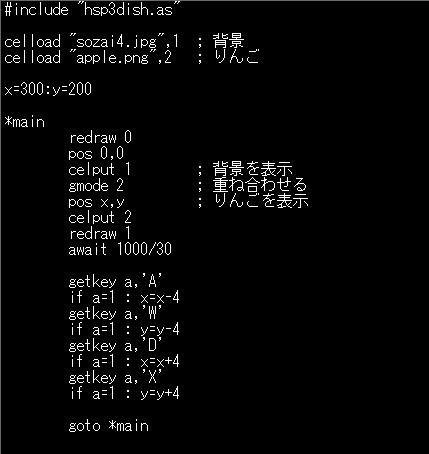
\includegraphics[keepaspectratio,width=10.61cm,height=11.229cm]{../../asset/image/s_move.png}
      \caption{move.hspの実行画面}
    \end{center}
\end{figure}

これは背景とりんごを表示するプログラムですが、リンゴを「A」「W」「D」「X」のキーを押して動かすことができます。何だかゲームみたいですね。

りんごをどのように動かしているのでしょうか。

いままでは、「x=x+2」のような行を入れて、１コマずつ動かしていました。

今度は、キーボードのボタンを押している時だけ、動くようにすればいいのです。

そのために、以前にも使った条件判断の仕組みを利用します。

キーボードが押されているかどうかを条件判断するために、新しい命令、getkeyの使い方を覚えておきましょう。

\deschspsyntax{getkey 変数, ‘キーの文字’}

と書くことで、指定した変数にキーが押されたかどうかが数値として代入されます。

たとえば、


\begin{lstlisting}[numbers=none]
getkey a, 'X'
\end{lstlisting}


を実行すると、「X」キーの\ruby{状態}{じょう|たい}で変数aの値が0か1になります。


\begin{itembox}[c]{getkeyの動作}
    「X」のキーが押されていない時は、変数aは0になります。\\「X」のキーが押されている時は、変数aは1になります。
\end{itembox}

キーの文字は、必ず大文字で’A’のように書く必要があるので注意してください。

文字の代わりにキーコードと呼ばれる数字を\ruby{指定}{し|てい}することで、特殊なキーの状態を知ることもできます。

\begin{center}
    \begin{tabular}{c|l} \hline
        キーコード & 実際のキー \\ \hline
        1 & マウスの左ボタン \\
        2 & マウスの右ボタン \\
        8 & [BACKSPACE] \\
        9 & [TAB] \\
        13 & [ENTER] \\
        16 & [SHIFT] \\
        17 & [CTRL] \\
        18 & [ALT] \\
        32 & スペースキー \\
        37 & カーソルキー[←] \\
        38 & カーソルキー[↑] \\
        39 & カーソルキー[→] \\
        40 & カーソルキー[↓] \\
        48〜57 & [0]〜[9]（メインキーボード） \\
        65〜90 & [A]〜[Z] \\
        96〜105 & [0]〜[9]（テンキー） \\
        112〜121 & ファンクションキー [F1]〜[F10] \\ \hline
    \end{tabular}
\end{center}

こうして代入された0か1の値を条件判断によって、やりたい内容を書くことで色々なことに応用ができます。

%2491
%2491

条件判断の方法をもう一度思い出してください。

if命令の使い方、ルールを覚えていますか?

\begin{itembox}[c]{HSPのルール}
    if命令により条件を判断することができます。ifの後にスペースに続けて\ruby{条件式}{じょう|けん|しき}を指定します。その後で「:」に続けて条件が正しい時に実行される命令を書きます。
\end{itembox}

\begin{center}
    (条件式はいくつか書き方があります)
\end{center}
\begin{center}
    \begin{tabular}{cl} \hline
        条件式 & 意味 \\ \hline
        変数名 = 数値 & 変数の内容と数値が同じである \\
        変数名 ! 数値 & 変数の内容と数値が同じではない \\
        変数名 {\textless} 数値 & 変数の内容より数値の方が数が大きい \\
        変数名 {\textgreater} 数値 & 変数の内容より数値の方が数が小さい \\ \hline
    \end{tabular}
\end{center}

下のプログラムがどのような意味か考えてみましょう。


\begin{lstlisting}[caption=プログラム,numbers=none]
getkey a, 'A'
if a=1 : x=x-4
\end{lstlisting}

最初は、条件判断の仕組みがわかりにくいかもしれませんが、プログラムの１行目から、コンピューターが実行することを想像しながら、1つ1つ確認することが大切です。

やがて、プログラムを見て、どのように動くのか想像ができるようになります。

最初はちょっと難しく感じるかもしれませんが、慣れれば誰でも理解できるようになります。

あせらず、わからない所はまわりの先生や友達に聞きながら、進んでいきましょう。

\subsection{例題に挑戦しよう}

ゲームが遊べた人は、以下の例題にも挑戦してみよう。

・センサーボードのボタンを使ってみよう

・照度センサーの値をもとに絵を動かそう

・照度センサーを使ったゲームを遊んでみよう

・センサーボードを使った応用例を考えてみよう


例題の考え方がわからない時は、近くのTAか先生に聞いてください。

わからない所は、そのままにせず、必ず答えを見つけてから先に進みましょう。

%2586
%2586
\newpage
\subsection{\useOmetoiExample　センサーボードの入力を使ってみよう}


\exampleinduction

キーボードの代わりにセンサーボードのボタンを使って絵を動かしてみましょう。

move.hspのプログラムを改造して、センサーボードのボタンで絵を動かせるようにしましょう。

\begin{lstlisting}[caption=move.hspのプログラム]
#include "hsp3dish.as"

    celload "sozai4.jpg",1  ; 背景
    celload "apple.png",2   ; りんご

    x=300:y=200

*main
    redraw 0
    pos 0,0
    celput 1        ; 背景を表示
    gmode 2         ; 重ね合わせる
    pos x,y         ; りんごを表示
    celput 2
    redraw 1
    await 1000/30

    getkey a,'A'
    if a=1 : x=x-4
    getkey a,'W'
    if a=1 : y=y-4
    getkey a,'D'
    if a=1 : x=x+4
    getkey a,'X'
    if a=1 : y=y+4

    goto *main
\end{lstlisting}

\exampleanswer

以前に取り上げた、GPIOの番号とその役割を思い出してみてください。


\begin{figure}[H]
    \begin{center}
      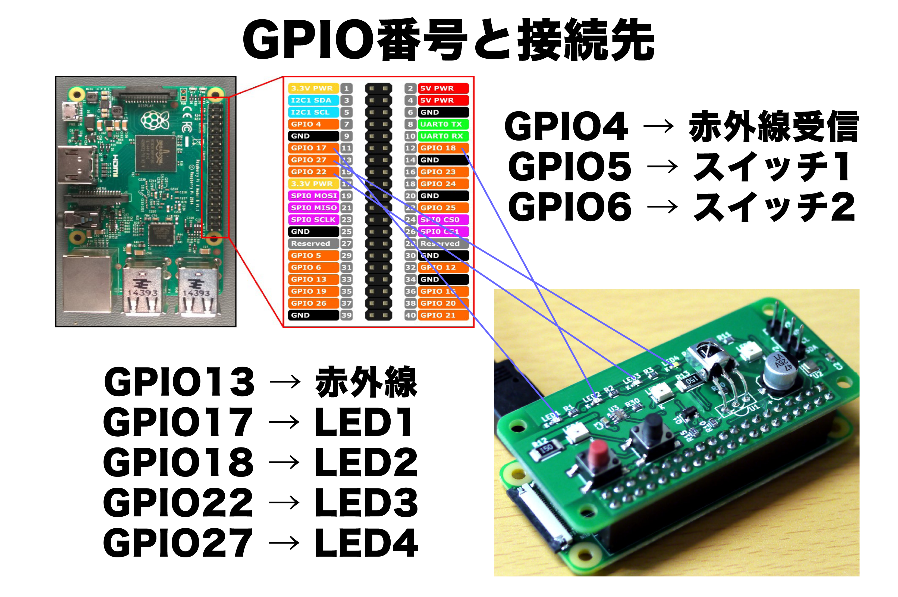
\includegraphics[keepaspectratio,width=10.372cm,height=6.89cm]{../../asset/image/s_gpio.png}
    \end{center} .
\end{figure}

スイッチの状態などを知る場合は、gpioinという関数を使います。

\deschspsyntax{変数 = gpioin(GPIO番号)}

と書くことで、指定されたGPIO番号のスイッチがONかOFFかを調べることができます。

変数には0か1の数字が代入されるので、条件判断を行うif命令で違う動作をさせることができます。


\begin{lstlisting}[numbers=none]
a = gpioin(5)
if a=0 : x=x-4
\end{lstlisting}

のように書くことで、変数aが0の時だけ「x=x-4」を実行させることができます。


以下のようにプログラムを改造することで、センサーボードのボタンを条件判断で使うことができます。

\begin{lstlisting}[numbers=none,caption=条件判断でセンサーボードのボタンを使う]
a=gpioin(5)
if a=0 : x=x-4
a=gpioin(6)
if a=0 ; x=x+4
getkey a, 'W'
if a=1 : y=y-4
getkey a, 'X'
if a=1 : y=y+4
\end{lstlisting}

改造ができたらTAや周りの友達にも見せてあげましょう。


以前に\ruby{乱数}{らん|すう}の使い方を学習したことを思い出してみましょう。

「x=rnd(640)」は、0〜639(640通り)までのバラバラな数字を変数xに代入します。

このような書き方を「\ruby{乱数}{らん|すう}」と呼んでいます。

\begin{figure}[H]
    \begin{center}
      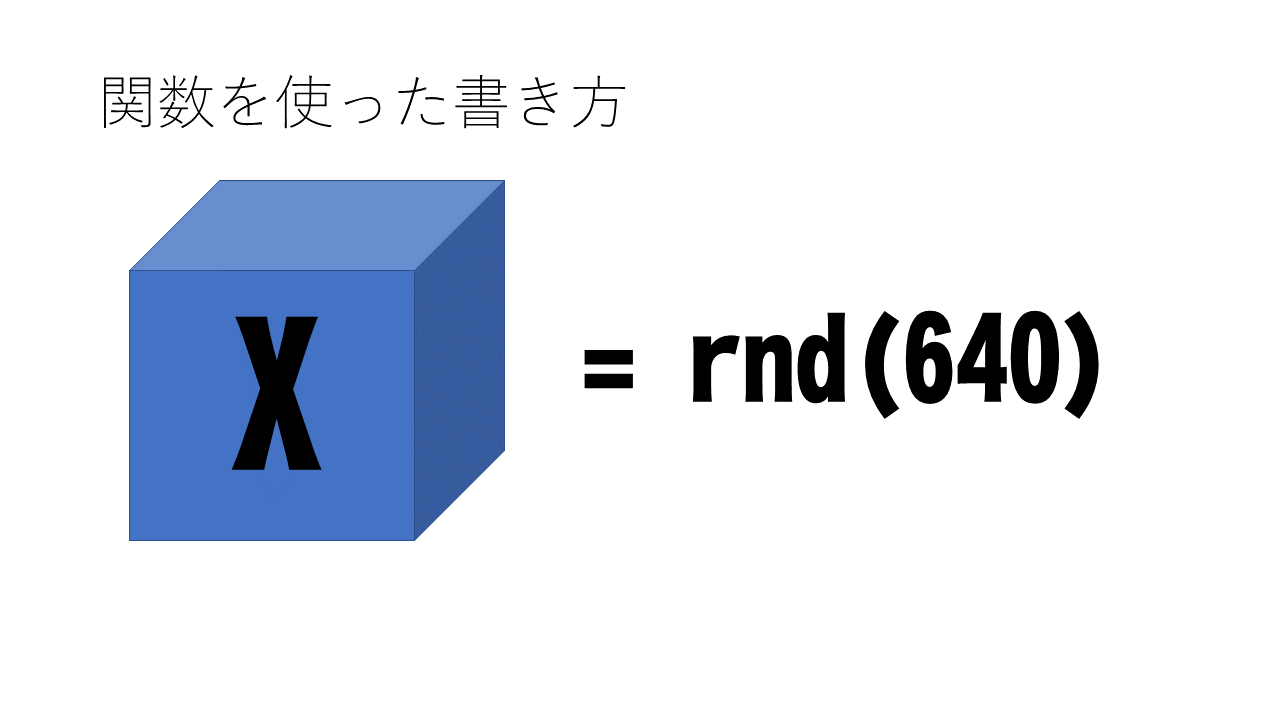
\includegraphics[keepaspectratio,width=11.906cm,height=5.662cm]{../../asset/image/s_rnd.png}
    \end{center}
\end{figure}

\begin{itembox}[c]{HSPのルール}
    \begin{itemize}
        \item 「変数=rnd(乱数の最大値)」でバラバラな数字を得ることができる
        \item 関数は、「変数=関数(パラメーター)」という書き方で使うことができる
    \end{itemize}
\end{itembox}

乱数が代入された変数を条件判断することで、でたらめな動きをする絵を作ることもできます。

余裕がある人は、乱数を使った動きにも挑戦してみましょう。

%2720
%2720
\newpage
\subsection{\useOmetoiExample　\ruby{照度}{しょう|ど}センサーの値をもとに絵を動かそう}

\exampleinduction

センサーボードのボタンだけでなく、\ruby{照度}{しょう|ど}センサーを使うこともできます。

照度センサーがどのような機能を持っているか、確認しておきましょう。


ファイル→「開く」メニューから「luxmove.hsp」を読み込んでください。

[F5]キーで実行すると、照度センサーの値が表示されると同時に小さな絵が動きます。

\begin{lstlisting}[caption=luxmove.hspのプログラム]
#include "hsp3dish.as"
#include "rpz-gpio.as"

        redraw 0
        mes "Reset..."
        redraw 1

        celload "tamane_s1.png",1
        geti2c_lux_init

*main
        geti2c_lux
        x=rpz_lux/32
        y=60

        redraw 0
        color 255,255,255:boxf
        color 0,0,0:pos 0,0:mes "="+rpz_lux
        pos x,y
        gmode 2
        celput 1,0,0.5,0.5

        redraw 1
        await 1000/30
        goto *main
\end{lstlisting}

左上に表示されている数値が照度センサーの値です。

明るい時ほど大きい数字になるのがわかりますか?

自分の手でセンサーを覆ったり、光を当ててみたりしながら値が変わることを確認してみましょう。

確認ができたら、move.hspのプログラムを改造して、りんごの絵を照度センサーの値によって動かせるようにしてみましょう。


\exampleanswer


「geti2c\_lux\_init」命令を最初に入れて１回だけ\ruby{初期化}{しょ|き|か}(準備)を行います。

その後、一定時間ごとに「geti2c\_lux」命令を実行することで、rpz\_luxという変数にセンサーの値が代入されます。

後は、rpz\_luxという変数の値をもとにプログラムで\ruby{処理}{しょ|り}を行います。

改造ができたらTAや周りの友達にも見せてあげましょう。

%2785
%2785
\newpage
\subsection{\useOmetoiExample　照度センサーを使ったゲームを遊んでみよう}

\exampleinduction


アイデア\ruby{次第}{し|だい}で、キーボードだけでなく、センサー\ruby{類}{るい}を使ってゲームのようにすることができます。

光センサーを使ったゲームを動かしてみましょう。


スクリプトエディタの、ファイル→「開く」メニューから「catch.hsp」を読み込んで実行してみてください。


\exampleanswer

センサーボードの光センサーから得た値を使って絵を動かしています。光センサーを手で\ruby{覆}{おお}ったり、\ruby{離}{はな}したりしてどうなるか確認してみましょう。

光センサーが暗くなった時には、キャラクターが左に移動します。光センサーが明るくなった時には、キャラクターが右に移動します。


\begin{figure}[H]
    \begin{center}
      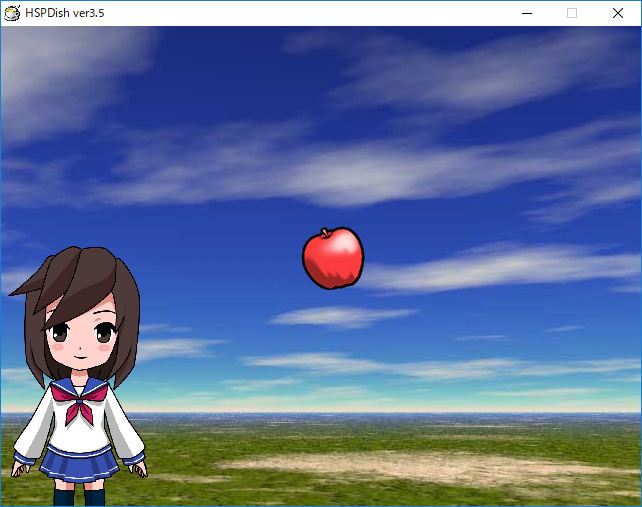
\includegraphics[keepaspectratio,width=11.269cm,height=8.89cm]{../../asset/image/s_catch.png}
      \caption{catch.hspの実行画面}
    \end{center}
\end{figure}

うまくキャラクターを移動させて、上から落ちてくるリンゴをキャッチしてみましょう。

これは、いままでの応用ですが、センサーと動きのある画面を組み合わせるだけでも、面白いものが作れるはずです。gpio命令で、LEDを光らせたり、スイッチを読み取ったりということと、変数・条件判断を組み合わせれば、さらに\ruby{応用範囲}{おう|よう|はん|い}が広がります。

%2844

%2844
\newpage
\subsection{\useOmetoiExample　センサーボードを使った応用例を考えてみよう}


\exampleinduction

今まで覚えてきたことを組み合わせて、何ができるか考えてみましょう。家に帰ってから、考えてみて答えを書いてきてください。センサーボードで何ができるか、プログラムでどんなことができるか、もう一度思い出してみて、考えてみましょう。

考えがまとまらない人は、いままでに動かしたプログラムを改造してみたいこと、センサーボードでやってみたいことを書いてみましょう。実際にプログラムを作る必要はありません。いっぱい考えついた人は、例題4-16と例題4-17の答えの欄に書いてみましょう。

大切なことは、自分で何でも試してみることです。わからないことがあっても、実際に実行すれば結果がわかります。立ち止まらずに、どうなるか想像しながらプログラムを書いて実行することが、早く\ruby{上達}{じょう|たつ}するコツになります。それでもわからない時は、先生に聞いてみましょう。

\exampleanswer

自分で考えた\ruby{応用例}{おう|よう|れい}を下に書いておきましょう。

応用例ができたら、今まで覚えてきた命令でできることか考えてみましょう。

実際に作れる人は、自分でプログラムを作ってみてください。

%2879

%2879
\newpage
\subsection{\useOmetoiExample　センサーボードの応用例をもっと考えてみよう(1)}

\exampleanswer

%2909
%2909
\newpage
\subsection{\useOmetoiExample　センサーボードの応用例をもっと考えてみよう(2)}

\exampleanswer


% Last Part:
%2942
\end{document}
